\documentclass[border=10pt,multi=page]{standalone}
\usepackage{pgf}
\usepackage{tikz}
\usetikzlibrary{arrows.meta}

\usetikzlibrary{arrows}
\usetikzlibrary{calc}
\usetikzlibrary{shapes}
\usetikzlibrary{trees}
\tikzset{>=stealth'}

% for pic 1
\usetikzlibrary{automata}

\begin{document}


\begin{page}

%pic 1
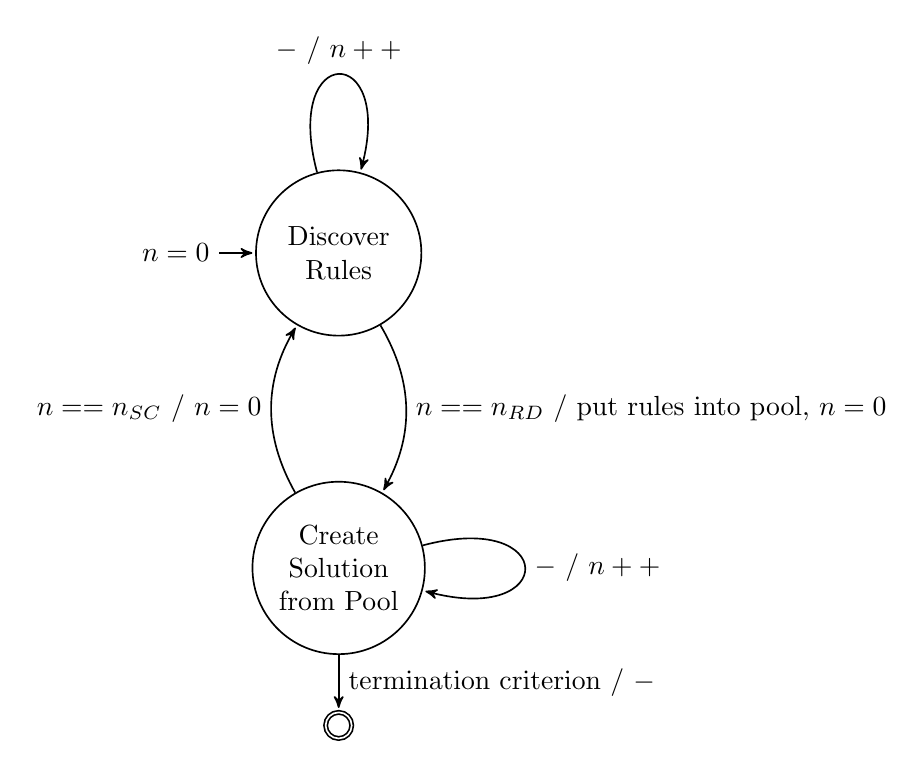
\begin{tikzpicture}[remember picture,->,>=stealth',shorten >=1pt,auto,node distance=4cm,semithick,initial text=${n=0}$]
  \tikzstyle{every state}=[fill=none,draw=black,text=black,align=center]
  

  \node[initial,state,minimum size=2.1cm] (D)                    {Discover\\ Rules};
  \node[state,minimum size=2.1cm]         (C) [below of=D]       {Create\\ Solution\\ from Pool};
  \node[state,accepting,yshift=2cm,minimum size=0.1cm](T)[below of=C]		  {};

  \path (D) edge[loop above] node {$-$ / $n++$}	(D)
            edge[bend left]	node[align=right] {$n==n_{RD}$ / put rules into pool, $n=0$}	(C)
		(C) edge[bend left] node[align=right] {$n==n_{SC}$ / $n=0$}	  	(D)
			edge[loop right] node {$-$ / $n++$}		(C)
			edge			  node[align=center] {termination criterion / $-$}		(T);
\end{tikzpicture}

\end{page}


\end{document}